\begin{frame}
\frametitle{NLS: oN-Line System}
\begin{itemize}
	\item 1960s
	\item Doug Engelbart, Stanford Research Institute
	\item Ziel war es "den menschlichen Intellekt zu erweitern"
	\begin{itemize}
		\item Computer zur direkten Interaktion
		\item Computer Bildschirme zur Darstellung von Text
	\end{itemize}
	\item Terminal
\end{itemize}

\begin{figure}[htbp]
	\centering
	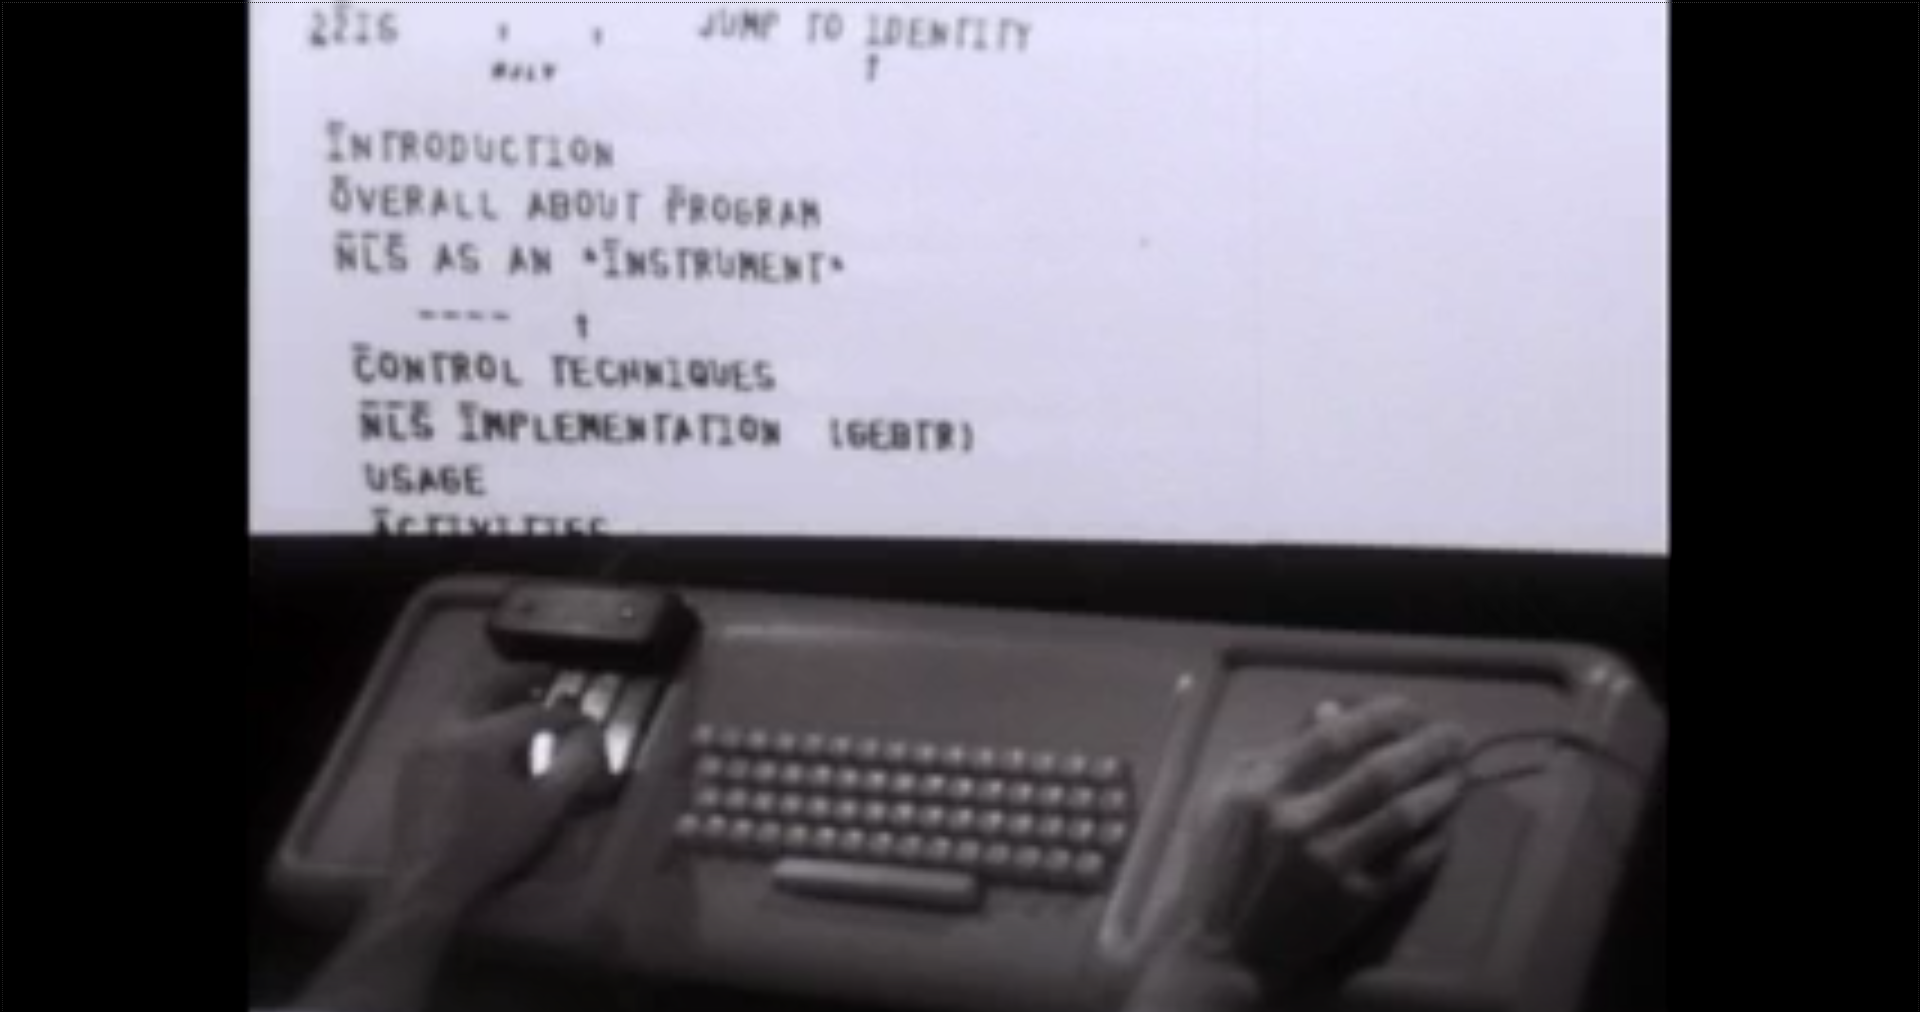
\includegraphics[width=0.7\textwidth]{images/nls}
\end{figure}

\end{frame}

\begin{frame}
\frametitle{NLS: oN-Line System}
\framesubtitle{Funktionen}
	\begin{itemize}
		\item Userinterface / Bedienmöglichkeiten
		\begin{itemize}
			\item Maus
			\item 5-Finger Tastatur
			\item Interaktives Textbearbeiten
		\end{itemize}
		\item Links / Strukturen
		\begin{itemize}
			\item Dokumente sind hierarchische strukturiert
			\item Jedes Segment hat eine ID
			\item Jede ID kann verlinkt werden
			\item Labels können verlinkt werden
		\end{itemize}
	\end{itemize}
\end{frame}
